\subsection{Типовые звенья непрерывных систем, частотные характеристики типовых звеньев}

Обычно система управления состоит из отдельных блоков, каждый из которых описывается уравнениями низкого порядка (первого и второго). Для понимания работы системы в целом желательно хорошо представлять, как ведут себя ее отдельные элементы. Для построения ЛАФЧХ передаточную функцию системы зазбивают на простейшие сомножители и строят характеристику для всей системы как сумму  ЛАЧХ и ЛФЧХ отдельных звеньев.

\begin{enumerate}
    \item Пропорциональное (безъинерционное) звено
    \begin{figure}[!h]
        \begin{minipage}[!h]{0.5\linewidth}
            \centering{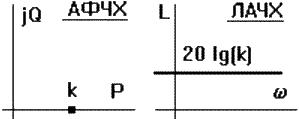
\includegraphics[width=1\linewidth]{images/links/pl.png}}
        \end{minipage}
        \begin{minipage}[!h]{0.5\linewidth}
            \begin{gather}
                W(s) = k, \quad W(j \omega) = k, \quad k \ne 0, \\
                \text{AЧХ и ФЧХ:\:\:}
                A(\omega) = k, \quad \phi(\omega) = 0, \\
                \text{ЛАФЧХ:\:\:}
                \begin{cases}
                    L(\omega) = 20 \log k \\
                    \phi(\omega) = 0.
                \end{cases}
            \end{gather}
        \end{minipage}
    \end{figure}

    \item Апериодическое звено
    \begin{figure}[!h]
        \begin{minipage}[!h]{0.5\linewidth}
            \centering{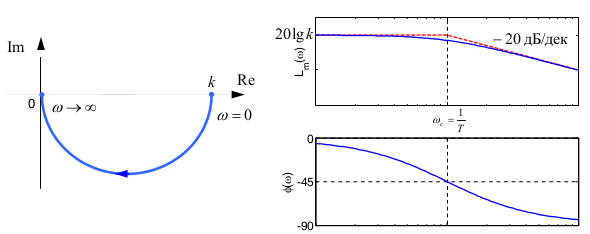
\includegraphics[width=1\linewidth]{images/links/al.png}}
        \end{minipage}
        \begin{minipage}[!h]{0.5\linewidth}
            \begin{gather}
                W(s) = \cfrac{k}{Ts + 1} = \cfrac{k - j k T \omega}{T^2 \omega^2 + 1}, \quad k \ne 0, T > 0 \\
                \text{AЧХ и ФЧХ:\:\:}
                A(\omega) = \cfrac{k}{\sqrt{T^2 \omega^2 + 1}}, \\ 
                \phi(\omega) = \arctan{\cfrac{ImW}{ReW}} = -\arctan{T \omega}, \\
                \text{ЛАФЧХ:\:\:}
                \begin{cases}
                    L(\omega) = 20 \log A(\omega) = -20 \log \sqrt{1+T^2 \omega^2} \\
                    \phi(\omega) = -\arctan{T \omega}.
                \end{cases}
            \end{gather}
        \end{minipage}
    \end{figure}
    
    \item Интегрирующее звено
    \begin{figure}[!h]
        \begin{minipage}[!h]{0.5\linewidth}
            \centering{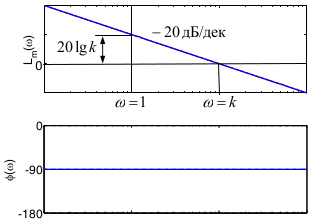
\includegraphics[width=1\linewidth]{images/links/il.png}}
        \end{minipage}
        \begin{minipage}[!h]{0.5\linewidth}
            \begin{gather}
                W(s) = \cfrac{k}{Ts} = \cfrac{k}{T j \omega}, \quad k \ne 0, T > 0 \\
                \text{AЧХ и ФЧХ:\:\:}
                A(\omega) = \cfrac{k}{T \omega}, \\ 
                \phi(\omega) = -\arctan{(-\infty)} = -\cfrac{\pi}{2}, \\
                \text{ЛАФЧХ:\:\:}
                \begin{cases}
                    L(\omega) = -20 \log T \omega \\
                    \phi(\omega) = -\cfrac{\pi}{2}.
                \end{cases}
            \end{gather}
        \end{minipage}
    \end{figure}
    
    \item Колебательное звено
    \begin{figure}[!h]
        \begin{minipage}[!h]{0.5\linewidth}
            \centering{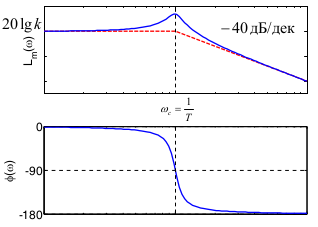
\includegraphics[width=1\linewidth]{images/links/gl.png}}
        \end{minipage}
        \begin{minipage}[!h]{0.5\linewidth}
            \begin{gather}
                W(s) = \cfrac{k}{T^2s^2 + 2 \xi T s + 1} = \cfrac{1-T^2\omega^2 - j 2 \xi T \omega}{4 \xi^2 T^2 \omega^2 + (1 - T^2 \omega^2)^2}, \\
                \text{AЧХ и ФЧХ:\:\:}
                A(\omega) = \cfrac{k}{\sqrt{4 \xi^2 T^2 \omega^2 + (1 - T^2 \omega^2)^2}}, \\ 
                \phi(\omega) = -\arctan{\cfrac{2 \xi T \omega}{1 - T^2 \omega^2}}, \\
                \text{ЛАФЧХ:\:\:}
                \begin{cases}
                    L(\omega) = -20 \log \sqrt{4 \xi^2 T^2 \omega^2 + (1 - T^2 \omega^2)^2} \\
                    \phi(\omega) = -\arctan{\cfrac{2 \xi T \omega}{1 - T^2 \omega^2}}.
                \end{cases}
            \end{gather}
        \end{minipage}
    \end{figure}
    
    \item Идеальное дифференцирующее звено
    \begin{figure}[!h]
        \begin{minipage}[!h]{0.5\linewidth}
            \centering{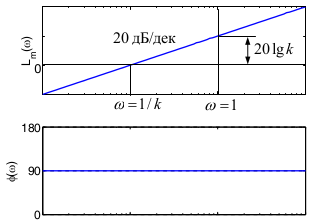
\includegraphics[width=1\linewidth]{images/links/dl.png}}
        \end{minipage}
        \begin{minipage}[!h]{0.5\linewidth}
            \begin{gather}
                W(s) = k s = k j \omega, \\
                \text{AЧХ и ФЧХ:\:\:}
                A(\omega) = k \omega, \\ 
                \phi(\omega) = \cfrac{\pi}{2}, \\
                \text{ЛАФЧХ:\:\:}
                \begin{cases}
                    L(\omega) = 20 \log(j k \omeg) \\
                    \phi(\omega) = \cfrac{\pi}{2}.
                \end{cases}
            \end{gather}
        \end{minipage}
    \end{figure}

\end{enumerate}


